\documentclass[12pt]{article}

% Packages for enhanced typesetting and functionality
\usepackage{amsmath, amssymb, amsthm}      % Maths symbols and environments
\usepackage{graphicx}                      % For including images
\usepackage{fancyhdr}                      % For header and footer customisation
\usepackage{geometry}                      % For margin customisation
\usepackage[colorlinks=true, linkcolor=blue, urlcolor=blue, citecolor=blue]{hyperref} % Clickable links
\usepackage{xcolor}                        % For coloured text
\usepackage{tikz}                          % For drawing diagrams and flowcharts
\usepackage{algorithm}                     % For algorithms
\usepackage[noend]{algpseudocode}          % For algorithm pseudocode
\usepackage{makecell}

% Page layout settings
\geometry{margin=2cm}
\setlength{\parindent}{0pt}
\setlength{\parskip}{1ex}

% Header and footer
\pagestyle{fancy}
\fancyhf{}
\setlength{\headheight}{15pt}
\fancyhead[L]{Comparative Metaheuristic Strategies}
\fancyhead[R]{Max Hart}
\fancyfoot[C]{\thepage}

\begin{document}

% Title Page
\begin{titlepage}
    \centering
    \vspace*{1cm}
    
    % University logo (adjust image file as needed)
    
\includegraphics[width=0.4\textwidth]{images/UoB.jpg}\par\vspace{1cm}
    
    {\LARGE\bfseries Comparative Metaheuristic Strategies\par for Airline Crew Scheduling\par}
    \vspace{0.5cm}
    {\Large A Study of Simulated Annealing and\par Genetic Algorithm Approaches\par}
    \vspace{0.75cm}
    
    {\large Evolutionary Computation\par}
    \vspace{1.5cm}
    
    {\large\textbf{Author:} Max Hart\par}
    \vspace{0.3cm}
    {\normalsize \href{mailto:mah422@student.bham.ac.uk}{mah422@student.bham.ac.uk}\par}
    \vspace{1.5cm}
    
    {\large\textbf{Professors:} Dr Shan He \& Dr Per Kristian Lehre\par}
    \vspace{1cm}
    
    {\large \today\par}
    
\end{titlepage}

\tableofcontents

\newpage

\section{Introduction}

The airline crew scheduling problem is a complex optimisation challenge, in which it is often framed as a Set Partitioning Problem (SPP).
In this setup, we must have each flight leg assigned to exactly one valid crew rotation. This must be done while satisfying various operational constraints. 
Due to the rapid growth in the number of possible assignments in comparison to the problem size, exact methods can struggle to scale.
This has led to the exploration of metaheuristic algorithms that offer practical, feasible (and often near-optimal) solutions within reasonable time.
These algorithms are particularly well-suited to the SPP, as they can efficiently navigate the vast solution space and balance the trade-offs between cost and constraint satisfaction.

In this project, we implement three such algorithms from scratch:
\begin{itemize}
    \item \textbf{Simulated Annealing (SA)}
    \item \textbf{Standard Binary Genetic Algorithm (BGA)}
    \item \textbf{Improved Binary Genetic Algorithm (BGA)}
\end{itemize}

We will test each of these algorithms for 30 runs on three instances from the OR-Library (sppnw41, sppnw42, sppnw43) and compare their performance in terms of feasibility, solution cost and overall robustness.
Each algorithm progressively improves in sophistication, with the Improved BGA incorporating several problem-specific enhancements to boost efficiency and constraint satisfaction. 
Specifically, we draw on ideas from Chu and Beasley~\cite{ChuAndBeasley1998} and Runarsson and Yao~\cite{RunarssonYao2000}, including pseudo-random initialization, heuristic improvement operators, and stochastic ranking for constraint handling.

Our main objective throughout this report is to investigate how these metaheuristic techniques will manage the complex challenges of the SPP, and to provide a comprehensive comparison of their performance.
Through this, we aim to gain insights into the strengths and weaknesses of each algorithm, and to identify the most effective strategies for solving airline crew scheduling problems.

\section{Metaheuristic Algorithms for the SPP}

In this section, we will provide a comprehensive overview of the three metaheuristic algorithms developed for solving the SPP. Each algorithm has been implemented from scratch in Python and is designed to find high-quality solutions to the airline crew scheduling problem.
For each algorithm, we will provide a brief introduction outlining its underlying principles and technical merits, followed by the corresponding pseudocode. Detailed flowcharts will be presented on subsequent pages to visually encapsulate the step-by-step processes. 
This thorough explanation is intended to clarify both the operational mechanics and the innovative aspects of our methods. 

\newpage

\subsection{Simulated Annealing}
Simulated Annealing is a local search technique that iteratively improves a candidate solution by exploring its neighbourhood. It uses a temperature parameter to probabilistically accept inferior solutions, thereby enabling the algorithm to escape local optima. 
This simple yet effective approach balances exploration and exploitation through gradual cooling.

\subsubsection{Pseudocode for Simulated Annealing}
The pseudocode below outlines the Simulated Annealing algorithm for the SPP, detailing random solution initialization, neighbour generation via bit-flipping, acceptance via direct improvement or the Metropolis criterion, and temperature cooling.

\begin{algorithm}[htbp]
  \caption{SimulatedAnnealing(\(T\), \(\alpha\), maxIter, penaltyFactor)}
  \label{alg:simulated_annealing}
  \begin{algorithmic}[1]
    \State \(\textbf{Initialisation:}\)
    \State \(x \gets \text{RandomSolution}()\) \Comment{Generate a random binary solution}
    \State \(F(x) \gets \text{PenaltyFitness}(x,\, \text{penaltyFactor})\) \Comment{Cost + coverage violations * penalty}
    \State \(x_{\text{best}} \gets x\); \quad \(F_{\text{best}} \gets F(x)\)

    \For{\(iter = 1\) to \(\text{maxIter}\)}
      \State \(\textbf{Neighbour generation:}\)
      \State \(x' \gets \text{FlipOneRandomBit}(x)\) \Comment{Create neighbour by flipping exactly one bit}

      \State \(\textbf{Evaluate neighbour:}\)
      \State \(F(x') \gets \text{PenaltyFitness}(x',\, \text{penaltyFactor})\)

      \If{\(F(x') < F(x)\)}
        \State \(x \gets x'\) 
        \Comment{If neighbour is better, accept it outright}
      \Else
        \State \(\Delta \gets F(x') - F(x)\)
        \Comment{Compute the increase in fitness}
        \State \(\textbf{Metropolis criterion:}\)
        \If{\(\text{rand}() < e^{-\Delta / T}\)}
          \State \(x \gets x'\) 
          \Comment{Accept worse solution with probability \(e^{-\Delta / T}\)}
        \EndIf
      \EndIf

      \State \(\textbf{Update global best:}\)
      \If{\(F(x) < F_{\text{best}}\)}
        \State \(x_{\text{best}} \gets x\); \quad \(F_{\text{best}} \gets F(x)\)
      \EndIf

      \State \(\textbf{Cool down:}\)
      \State \(T \gets \alpha \times T\)
    \EndFor
    
    \State \Return \(\bigl(x_{\text{best}},\, F_{\text{best}}\bigr)\)
  \end{algorithmic}
\end{algorithm}

\subsubsection{Flowchart for Simulated Annealing}
The flowchart visually represents the step-by-step process of the Simulated Annealing algorithm, from initialisation and neighbour evaluation to acceptance decisions and temperature cooling.

\begin{figure}[htbp]
  \centering
  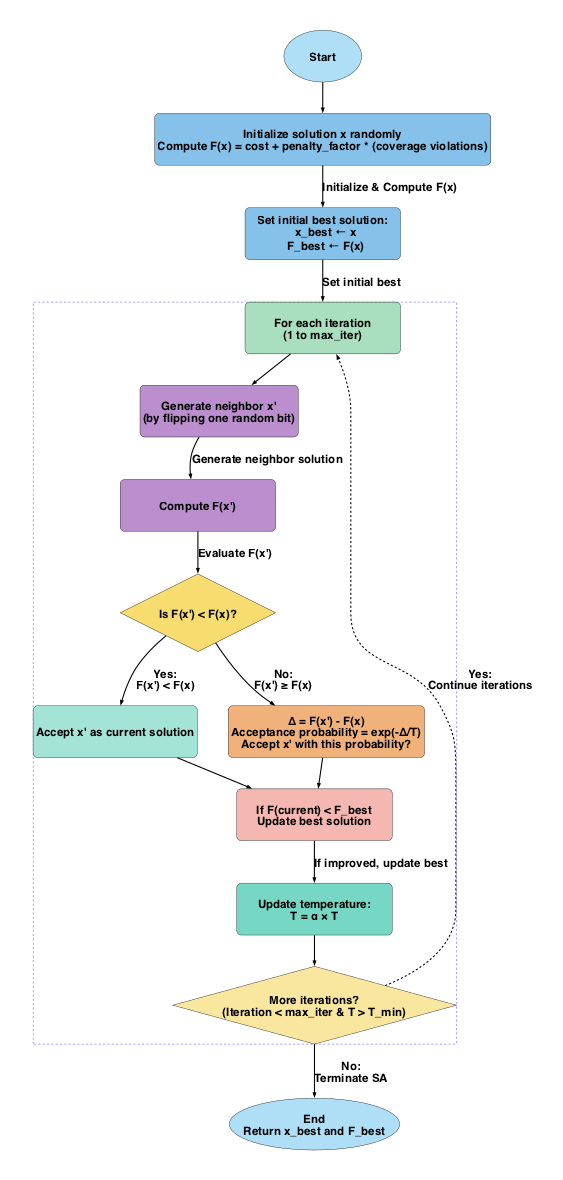
\includegraphics[width=0.60\textwidth]{images/simulated_annealing_flowchart.png}
  \caption{Flowchart of the Simulated Annealing Algorithm for the Set Partitioning Problem.}
  \label{fig:flowchart1}
\end{figure}

\newpage

\subsection{Standard Binary Genetic Algorithm}
The Standard Binary Genetic Algorithm is a population-based technique that evolves a set of candidate solutions using selection, crossover, and mutation operators. 
It utilises tournament selection to choose parents, applies one-point crossover to combine their genetic material, and uses bit-flip mutation to introduce variability. 
A penalty function is employed to combine the cost of a solution with constraint violations, ensuring that feasibility is encouraged over generations. 
This method is well-suited for problems with discrete binary representations and offers robustness through its stochastic operations.

\subsubsection{Pseudocode for Standard BGA}
The pseudocode below outlines the Standard Binary Genetic Algorithm for the SPP, detailing population initialisation, tournament selection, crossover, mutation, and population update.

\begin{algorithm}[htbp]
  \caption{StandardBGA(\textit{popSize}, \textit{cxRate}, \textit{mutRate}, \textit{maxGens}, \textit{penaltyFactor}, \textit{tournK})}
  \label{alg:standard_bga}
  \begin{algorithmic}[1]
    \State \(\textbf{Initialise:}\)
    \State $P \gets \text{RandomPopulation}(\textit{popSize})$ 
      \Comment{Generate \(\textit{popSize}\) random binary solutions}
    \State $\text{EvaluateFitness}(P,\, \textit{penaltyFactor})$ 
      \Comment{Compute cost + penalty for each individual}
    \State $(\textit{xBest}, F_{\text{best}}) \gets \text{BestSolution}(P)$ 
      \Comment{Track best overall}

    \For{$g = 1 \to \textit{maxGens}$}
      \State $Q \gets \varnothing$ \Comment{Offspring population}
      \While{$|Q| < \textit{popSize}$}
        \State $p_1 \gets \text{TournamentSelect}(P, \textit{tournK})$ 
          \Comment{Select parent 1}
        \State $p_2 \gets \text{TournamentSelect}(P, \textit{tournK})$ 
          \Comment{Select parent 2}
        
        \If{$\text{rand}() < \textit{cxRate}$}
          \State $(c_1, c_2) \gets \text{OnePointCrossover}(p_1, p_2)$
          \Comment{Split at random point and swap tails}
        \Else
          \State $c_1 \gets p_1,\quad c_2 \gets p_2$ 
          \Comment{No crossover; children are copies}
        \EndIf

        \State $\text{Mutate}(c_1,\, \textit{mutRate})$
        \State $\text{Mutate}(c_2,\, \textit{mutRate})$
          \Comment{Bit-flip mutation with prob = \textit{mutRate}}

        \State $\text{EvaluateFitness}(\{c_1, c_2\}, \textit{penaltyFactor})$
          \Comment{Compute cost + penalty of each child}
        
        \State $Q \gets Q \cup \{\,c_1,\,c_2\}$
      \EndWhile

      \State $P \gets Q$ \Comment{Replace old population with offspring}
      \State $(\textit{xCurrBest}, F_{\text{currBest}}) \gets \text{BestSolution}(P)$
      \If{$F_{\text{currBest}} < F_{\text{best}}$}
        \State $\textit{xBest} \gets \textit{xCurrBest}$,\quad $F_{\text{best}} \gets F_{\text{currBest}}$
          \Comment{Update global best if improved}
      \EndIf
    \EndFor
    
    \State \Return $(\textit{xBest},\, F_{\text{best}})$ 
      \Comment{Best solution found}
  \end{algorithmic}
\end{algorithm}

\subsubsection{Flowchart for Standard BGA}
The flowchart provides a visual overview of the Standard BGA’s iterative process, from offspring generation to re-ranking and best solution update.

\begin{figure}[htbp]
  \centering
  % Adjust the width as needed, e.g., 0.9\textwidth fills most of the page width
  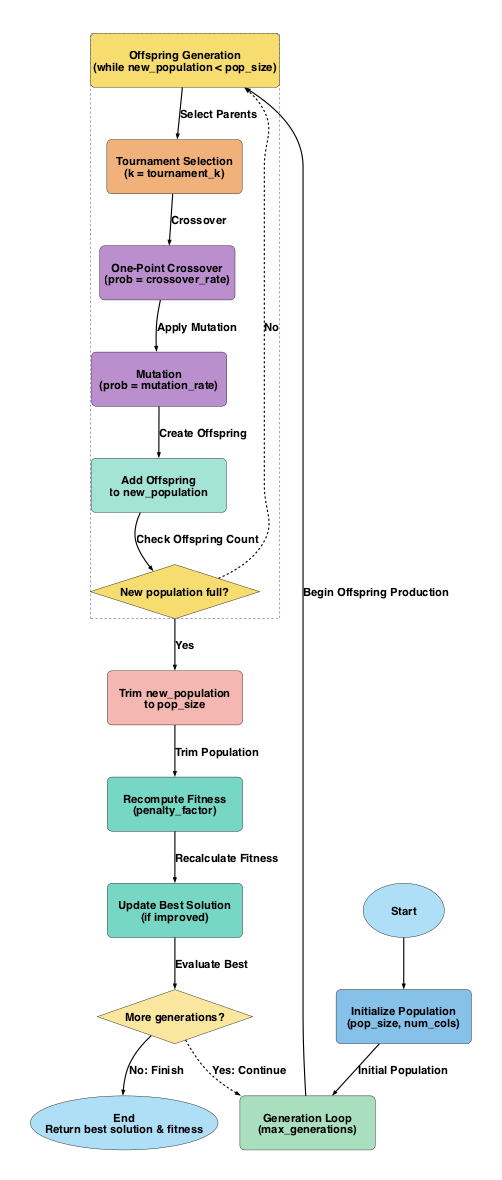
\includegraphics[width=0.53\textwidth]{images/standard_bga_flowchart.png}
  \caption{Flowchart of the Standard Binary Genetic Algorithm for the Set Partitioning Problem.}
  \label{fig:flowchart2}
\end{figure}

\newpage

\subsection{Improved Binary Genetic Algorithm}
The Improved Binary Genetic Algorithm extends the standard Binary Genetic Algorithm by integrating several problem-specific enhancements. It begins with a pseudo–random initialisation that aims to reduce over–coverage in the initial population. The algorithm then incorporates a stochastic ranking procedure that probabilistically balances cost and constraint violation, allowing for a more flexible handling of infeasible solutions. Adaptive mutation is employed to reintroduce promising genetic material, and a DROP/ADD heuristic improvement operator repairs infeasible solutions. These enhancements, inspired by Chu \& Beasley~\cite{ChuAndBeasley1998} and Runarsson \& Yao~\cite{RunarssonYao2000}, make the Improved BGA particularly robust for the SPP. Overall, this algorithm offers a more sophisticated search mechanism by blending global search operators with domain-specific repairs.

\subsubsection{Pseudocode for Improved BGA}
The pseudocode below describes the Improved Binary Genetic Algorithm for the SPP, integrating pseudo–random initialisation, stochastic ranking, adaptive mutation, and heuristic repair.

\begin{algorithm}[htbp]
  \caption{ImprovedBGA(\textit{popSize}, \textit{maxGens}, \(\textit{p}_{\mathrm{stoch}}\), \dots)}
  \label{alg:improved_bga}
  \begin{algorithmic}[1]
    \State \(\textbf{Initialise:}\)
    \State $P \gets \text{PseudoRandomInit}(\textit{popSize})$ 
      \Comment{Chu \& Beasley [1] for partial coverage}
    \State $\text{EvaluateCostUnfitness}(P)$ 
      \Comment{For each individual, compute $(\mathrm{cost}, \mathrm{violations})$}
    
    \For{$g = 1 \to \textit{maxGens}$}
      \State $\text{StochasticRankSort}(P,\, \textit{p}_{\mathrm{stoch}})$ 
        \Comment{Runarsson \& Yao [2] sort by cost vs. unfitness}
      \State $O \gets \varnothing$ 
        \Comment{Offspring population}

      \While{$|O| < \textit{popSize}$}
        \State $(p_1, p_2) \gets \text{SelectParents}(P)$ 
          \Comment{Randomly pick two parents}
        \State $(c_1, c_2) \gets \text{UniformCrossover}(p_1, p_2)$ 
          \Comment{Exchange bits at random (50\% each)}
        
        \State $\text{AdaptiveMutation}(c_1, P)$ 
          \Comment{Bit-flip mutation + forced coverage}
        \State $\text{AdaptiveMutation}(c_2, P)$

        \State $\text{HeuristicImprove}(c_1)$ 
          \Comment{Repair via DROP/ADD (Chu \& Beasley [1])}
        \State $\text{HeuristicImprove}(c_2)$
        
        \State $\text{EvaluateCostUnfitness}(\{c_1, c_2\})$
        \State $O \gets O \cup \{c_1,\, c_2\}$
      \EndWhile

      \State $C \gets P \cup O$ 
        \Comment{Combine parents \& offspring}
      \State $\text{StochasticRankSort}(C,\, \textit{p}_{\mathrm{stoch}})$ 
        \Comment{Re-sort combined pop}
      \State $P \gets \text{Top}(C,\; \textit{popSize})$
        \Comment{Keep the best \textit{popSize}}
    \EndFor
    
    \State \Return $\text{BestFeasible}(P)$ 
      \Comment{Return best feasible (lowest cost, unfitness=0)}
  \end{algorithmic}
\end{algorithm}

\subsubsection{Flowchart for Improved BGA}
The flowchart visually maps the Enhanced BGA’s process, clearly highlighting its advanced offspring production and repair mechanisms.
\begin{figure}[htbp]
  \centering
  % Adjust the width as needed, e.g., 0.9\textwidth fills most of the page width
  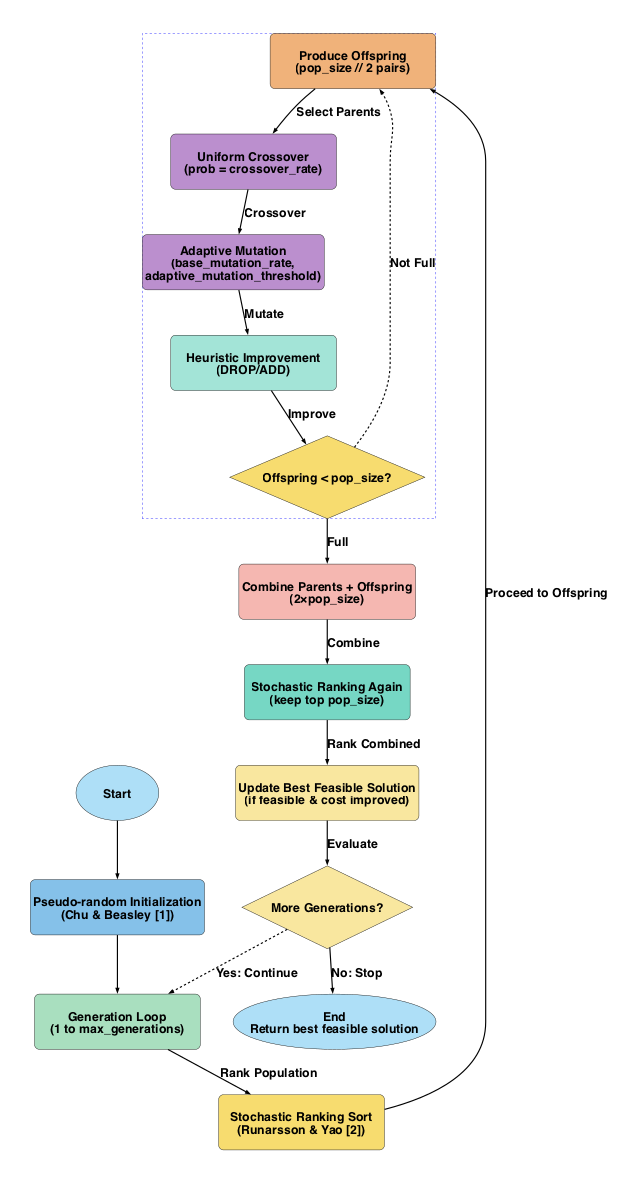
\includegraphics[width=0.70\textwidth]{images/improved_bga_flowchart.png}
  \caption{Flowchart of the Improved Binary Genetic Algorithm for the Set Partitioning Problem.}
  \label{fig:flowchart3}
\end{figure}

\newpage

\section{Benchmark Results}
\label{sec:benchmark_results}

In this section, we present the results obtained by our three algorithms---Simulated Annealing (SA), Standard BGA, and Improved BGA---on three different problem sets. Each subsection provides a table summarising performance metrics across 30 independent runs, focusing on feasibility and overall solution quality. In particular, we report the rate at which each method produces a feasible solution (\emph{Feas.\ Rate}), best/worst feasible cost, average feasible cost (with standard deviation), and average execution time (with standard deviation).

\subsection{Problem Set \texttt{sppnw41}}
\label{subsec:sppnw41}

We tested each algorithm for 30 independent runs on the \texttt{sppnw41} problem instance. 
Table~\ref{tab:sppnw41} shows the feasibility rate, along with best, worst, and mean feasible costs (plus standard deviation), as well as average run time (plus standard deviation) for each algorithm. 
All results are based on runs that reached feasibility (zero coverage violations). 
A brief description of the hyperparameters used in each method can be found below.

\vspace{1em}

\begin{table}[htbp]
  \centering
  \label{tab:sppnw41}
  \renewcommand{\arraystretch}{1.1}
  \begin{tabular}{lcccccc}
    \hline
    \textbf{Algorithm} & \makecell{Feas.\\Rate} & \makecell{Best\\Cost} & \makecell{Worst\\Cost} & \makecell{Mean\\Cost} & \makecell{Std.\\Dev.} & \makecell{Time\\(s) $\pm$ SD}\\
    \hline
    SA            
      & 12/30 
      & 18,066
      & 32,730 
      & 23,344
      & 4,002 
      & 0.082 $\pm$ 0.0008 \\
    Standard BGA 
      & 21/30 
      & 12,678 
      & 28,269 
      & 20,188 
      & 3,736 
      & 1.94 $\pm$ 0.07 \\
    Improved BGA 
      & 30/30 
      & 11,307 
      & 13,395 
      & 12,177 
      & 658 
      & 2.65 $\pm$ 0.05 \\
    \hline
  \end{tabular}
  \caption{Performance on \texttt{sppnw41} (30 runs). Feasible solutions have zero coverage violations.}
\end{table}

\paragraph{Hyperparameters.}
\vspace{-0.75em}
\begin{itemize}
    \item \textbf{Simulated Annealing (SA).} 
    Initial temperature $= 2000.0$, 
    cooling factor $\alpha = 0.99$, 
    maximum iterations $= 10,000$, 
    penalty factor $= 50000$. 
    \item \textbf{Standard BGA.}
    Population size $= 250$, 
    crossover rate $= 0.8$, 
    mutation rate $= 0.003$, 
    max generations $= 500$, 
    penalty factor $= 4800.0$, 
    tournament size $= 4$.
    \item \textbf{Improved BGA.}
    Population size $= 50$, 
    max generations $= 200$, 
    crossover rate $= 0.85$, 
    base mutation rate $= 0.03$, 
    stochastic rank $p = 0.45$, 
    adaptive mutation threshold $= 0.2$, 
    adaptive mutation count $= 2$.
\end{itemize}

\noindent
As shown, the Improved BGA achieves a 100\% feasibility rate and outperforms the other algorithms in terms of average feasible cost for this problem set, albeit with a slightly longer average run time.


\subsection{Problem Set \texttt{sppnw42}}
\label{subsec:sppnw42}

We tested each algorithm for 30 independent runs on the \texttt{sppnw42} problem instance. 
Table~\ref{tab:sppnw42} shows the feasibility rate, along with best, worst, and mean feasible costs (plus standard deviation), as well as average run time (plus standard deviation) for each algorithm. 
All results are based on runs that reached feasibility (zero coverage violations). 
A brief description of the hyperparameters used in each method can be found below.

\vspace{1em}

\begin{table}[htbp]
  \centering
  \label{tab:sppnw42}
  \renewcommand{\arraystretch}{1.1}
  \begin{tabular}{lcccccc}
    \hline
    \textbf{Algorithm} 
      & \makecell{Feas.\\Rate} 
      & \makecell{Best\\Cost} 
      & \makecell{Worst\\Cost} 
      & \makecell{Mean\\Cost} 
      & \makecell{Std.\\Dev.} 
      & \makecell{Time\\(s) $\pm$ SD}\\
    \hline
    \textbf{SA}          
      & 1/30 
      & 14,222
      & 14,222
      & 14,222
      & 0
      & 0.608 $\pm$ 0.000 \\
    \textbf{Standard BGA} 
      & 0/30
      & — 
      & —
      & —
      & —
      & — \\
    \textbf{Improved BGA} 
      & 30/30 
      & 7,666
      & 8,666
      & 7,927
      & 284
      & 19.28 $\pm$ 0.78 \\
    \hline
  \end{tabular}
  \caption{Performance on \texttt{sppnw42} (30 runs). Feasible solutions have zero coverage violations.}
\end{table}

\paragraph{Hyperparameters.}
\vspace{-0.75em}
\begin{itemize}
    \item \textbf{Simulated Annealing (SA).} 
    Initial temperature $= 5000.0$, 
    cooling factor $\alpha = 0.99$, 
    max iterations $= 10{,}000$, 
    penalty factor $= 100{,}000$. 
    \item \textbf{Standard BGA.}
    Population size $= 400$, 
    crossover rate $= 0.9$, 
    mutation rate $= 0.003$, 
    max generations $= 1000$, 
    penalty factor $= 10{,}000$, 
    tournament size $= 5$. 
    \item \textbf{Improved BGA.}
    Population size $= 30$, 
    max generations $= 400$, 
    crossover rate $= 0.85$, 
    base mutation rate $= 0.03$, 
    stochastic rank $p = 0.45$, 
    adaptive mutation threshold $= 0.25$, 
    adaptive mutation count $= 2$.
\end{itemize}

\noindent
As shown, the Standard BGA failed to reach feasibility in any run, while Simulated Annealing found a valid solution only once. By contrast, the Improved BGA maintained a $100\%$ feasibility rate and delivered competitive costs consistently.

\subsection{Problem Set \texttt{sppnw43}}
\label{subsec:sppnw43}

We tested each algorithm for 30 independent runs on the \texttt{sppnw43} problem instance. 
Table~\ref{tab:sppnw43} shows the feasibility rate, along with best, worst, and mean feasible costs (plus standard deviation), as well as average run time (plus standard deviation) for each algorithm. 
All results are based on runs that reached feasibility (zero coverage violations). 
A brief description of the hyperparameters used in each method can be found below.

\vspace{1em}

\begin{table}[htbp]
  \centering
  \label{tab:sppnw43}
  \renewcommand{\arraystretch}{1.1}
  \begin{tabular}{lcccccc}
    \hline
    \textbf{Algorithm} 
      & \makecell{Feas.\\Rate} 
      & \makecell{Best\\Cost} 
      & \makecell{Worst\\Cost} 
      & \makecell{Mean\\Cost} 
      & \makecell{Std.\\Dev.} 
      & \makecell{Time\\(s) $\pm$ SD}\\
    \hline
    \textbf{SA}          
      & 5/30
      & 11{,}996
      & 17{,}614
      & 14{,}600
      & 2{,}100
      & 0.57 $\pm$ 0.01 \\
    \textbf{Standard BGA} 
      & 0/30 
      & — 
      & —
      & —
      & —
      & — \\
    \textbf{Improved BGA} 
      & 30/30 
      & 8{,}974
      & 10{,}042
      & 9{,}517
      & 278
      & 21.78 $\pm$ 0.47 \\
    \hline
  \end{tabular}
  \caption{Performance on \texttt{sppnw43} (30 runs). Feasible solutions have zero coverage violations.}
\end{table}

\paragraph{Hyperparameters.}
\vspace{-0.75em}
\begin{itemize}
    \item \textbf{Simulated Annealing (SA).}
    Initial temperature $= 5000.0$, 
    cooling factor $\alpha = 0.99$, 
    max iterations $= 10{,}000$, 
    penalty factor $= 100{,}000$. 
    
    \item \textbf{Standard BGA.}
    Population size $= 400$, 
    crossover rate $= 0.9$, 
    mutation rate $= 0.003$, 
    max generations $= 1000$, 
    penalty factor $= 10{,}000$, 
    tournament size $= 5$. 
    
    \item \textbf{Improved BGA.}
    Population size $= 30$, 
    max generations $= 400$, 
    crossover rate $= 0.85$, 
    base mutation rate $= 0.03$, 
    stochastic rank $p = 0.56$, 
    adaptive mutation threshold $= 0.25$, 
    adaptive mutation count $= 2$.
\end{itemize}

\noindent
As indicated in Table~\ref{tab:sppnw43}, the Standard BGA again failed to produce any feasible solution, whereas Simulated Annealing identified a valid solution in only $16.7\%$ of runs. By contrast, the Improved BGA achieved a $100\%$ feasibility rate with a notably lower mean feasible cost.


\section{Discussion and Comparison}
\label{sec:discussion}


\section{Ranking Replacement vs. Stochastic Ranking}
\label{sec:ranking}
Both methods aim to balance cost and constraint satisfaction in the SPP, yet they differ in approach. The \textbf{Ranking Replacement} method (Chu \& Beasley, 1998) partitions the population deterministically into four subgroups based on fitness (cost) and unfitness (constraint violation). A new solution replaces an individual from the first non-empty subgroup (starting with those worst in both criteria), thereby steadily improving the overall population. This approach offers a clear structure but can be rigid as the balance between cost and constraint violation may evolve during the search.

In contrast, the \textbf{Stochastic Ranking} method (Runarsson \& Yao, 2000) uses a bubble-sort-like procedure where adjacent solutions are compared probabilistically—if at least one solution is infeasible, they are compared by cost with a set probability \(P\) (typically less than 0.5) and by unfitness otherwise. This allows for a more adaptive balance, enabling the search to explore infeasible regions as bridges between isolated feasible areas without rigid subgroup thresholds.

In summary, while both methods share the goal of guiding the search toward feasible, high-quality solutions, Ranking Replacement enforces a strict hierarchical structure, whereas Stochastic Ranking offers a flexible, adaptive mechanism that reduces the need for extensive parameter tuning.
\section{Conclusion}
This report has presented three advanced algorithms for solving airline crew scheduling problems: Simulated Annealing, a Standard Binary Genetic Algorithm, and an Improved Binary Genetic Algorithm incorporating problem-specific enhancements. Detailed, moderately sized flowcharts and refined pseudocode have been provided to elucidate each method's internal workings. Benchmark results and an in-depth discussion will be appended once experiments are complete. Furthermore, a comparative discussion on constraint-handling—contrasting ranking replacement and stochastic ranking—has been included, underscoring the adaptive advantages of the latter.

\newpage

\begin{thebibliography}{9}
\bibitem{ChuAndBeasley1998}
  P.~C. Chu and J.~E. Beasley, 
  \emph{Constraint Handling in Genetic Algorithms: The Set Partitioning Problem},
  Journal of Heuristics, 11:323--357, 1998.

\bibitem{RunarssonYao2000}
  T.~P. Runarsson and X. Yao, 
  \emph{Stochastic Ranking for Constrained Evolutionary Optimisation},
  IEEE Transactions on Evolutionary Computation, 4(3):284--294, 2000.
\end{thebibliography}

\end{document}